\section{Experiments}

\begin{figure}[t]
    \centering
    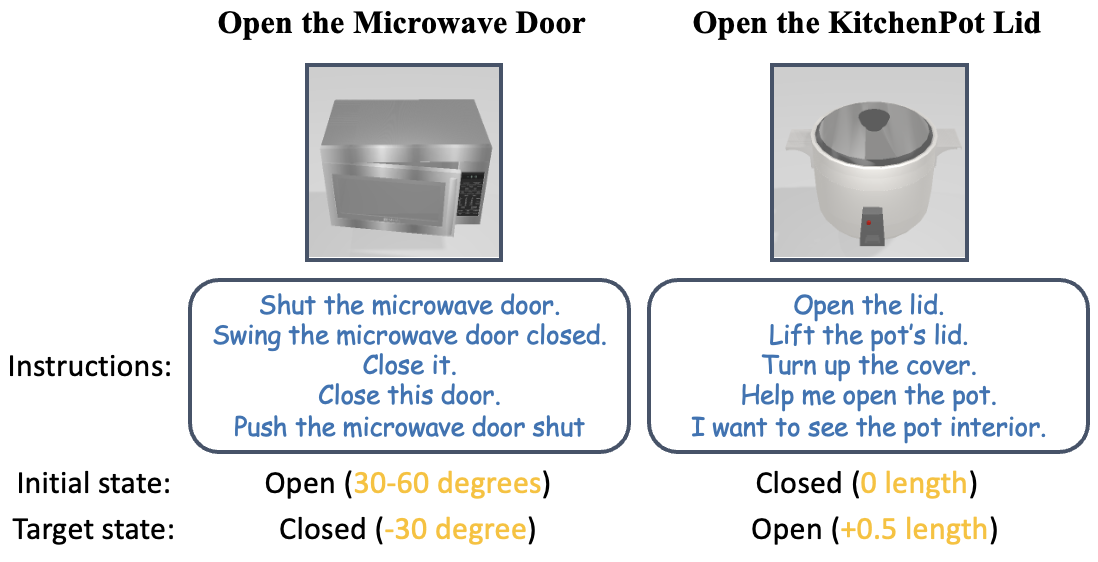
\includegraphics[width=.85\linewidth]{figures/sim_demo2.jpg}
    \caption{\textbf{Task examples for experiments in simulation.}}
    \label{fig:bench_demo}
    \vspace{-0.5cm}
\end{figure}

\begin{table*}[t]
    \centering
    \resizebox{2.\columnwidth}{!}{
\begin{tabular}{l|ccc|ccc|ccc|c|c|c}
\toprule
Category & \multicolumn{3}{c|}{Microwave} & \multicolumn{3}{c|}{StorageFurniture} & \multicolumn{3}{c|}{Cabinet} & KitchenPot & Remote & Blender \\ \midrule
Task ID & 1 & 2 & 3 & 4 & 5 & 6 & 7 & 8 & 9 & 10 & 11 & 12 \\ \midrule
VoxPoser$^*$\citep{huang2023voxposer} & - & - & 13.0 & - & - & 15.0 & - & - & 14.2 & - & - & - \\
GAPartNet$^*$\citep{geng2022gapartnet} & 87.5 & 75.5 & 58.6 & 53.3 & 76.9 & 81.3 & 50.0 & 66.3 & 73.8 & - & - & - \\
Ours & \textbf{98.0} & \textbf{96.0} &\textbf{94.1} & \textbf{83.3} & \textbf{80.0} &\textbf{95.0} & \textbf{79.3} & \textbf{89.6} & \textbf{83.1} &\textbf{85.7} & \textbf{60.7}& \textbf{42.9}\\ \bottomrule
\end{tabular}
}
\caption{\textbf{Success rates (\%) under language instructions.} Comparison between our method with VoxPoser \citep{huang2023voxposer} and GAPartNet\citep{geng2022gapartnet}. We evaluate 12 tasks with 6 different articulated objects. "-" means the task is not implemented by the baseline. GAPartNet$^*$ shares the same execution policy as our method, while VoxPoser$^*$ is adapted from the unofficial version of the authors.}
\vspace{-0.5cm}
\label{tab:main_results}
\end{table*}


\begin{table}[t]
    \centering
    \setlength{\tabcolsep}{3pt}
    \resizebox{\columnwidth}{!}{
    \begin{tabular}{l|cccc}
    \toprule
    Category & \#Task & \#Init. state & \#Tgt. state & \#Instruct. \\
    \midrule
    Microwave & 100 & 3 & 2 & 5 \\
    StorageFurniture & 40 & 3 & 2 & 5 \\
    Cabinet & 40 & 3 & 2 & 5 \\
    KitchenPot & 20 & 1 & 1 & 5 \\
    Remote & 18 & 1 & 1 & 5 \\
    Blender & 20 & 1 & 1 & 5 \\
    \bottomrule
    \end{tabular}}
    \caption{\textbf{Benchmark statistics.} For each object category, we created tasks that were randomly initialized.}
    \label{tab:bench_stat}
\end{table}


% \begin{figure*}[htbp]
% % \vspace{-1.5cm}
% \begin{minipage}[c]{0.60\linewidth}
% \vspace{-0.5cm}
% \resizebox{1.\columnwidth}{!}{
% \begin{tabular}{c|ccc|ccc|ccc|c|c|c}
% \label{tab:baseline}
% \hline
% Obj. Cat. & \multicolumn{3}{c|}{Microwave} & \multicolumn{3}{c|}{StorageFurniture} & \multicolumn{3}{c|}{Cabinet} & KitchenPot & Remote & Blender \\ \hline
% Task ID & \multicolumn{1}{c|}{1} & \multicolumn{1}{c|}{2} & 3 & \multicolumn{1}{c|}{4} & \multicolumn{1}{c|}{5} & 6 & \multicolumn{1}{c|}{7} & \multicolumn{1}{c|}{8} & 9 & 10 & 11 & 12 \\ \hline
% VoxPoser$^*$(\%) & \multicolumn{1}{c|}{-} & \multicolumn{1}{c|}{-} & 13.0 & \multicolumn{1}{c|}{-} & \multicolumn{1}{c|}{-} & 15.0 & \multicolumn{1}{c|}{-} & \multicolumn{1}{c|}{-} & 14.2 & - & - & - \\ \hline
% GAPartNet$^*$(\%) & \multicolumn{1}{c|}{87.5} & \multicolumn{1}{c|}{75.5} & 58.6 & \multicolumn{1}{c|}{53.3} & \multicolumn{1}{c|}{76.9} & 81.3 & \multicolumn{1}{c|}{50.0} & \multicolumn{1}{c|}{66.3} & 73.8 & - & - & - \\ \hline
% Ours(\%) & \multicolumn{1}{c|}{\textbf{98.0}} & \multicolumn{1}{c|}{\textbf{96.0}} &\textbf{ 94.1} & \multicolumn{1}{c|}{\textbf{83.3}} & \multicolumn{1}{c|}{\textbf{80.0 }} &\textbf{ 95.0} & \multicolumn{1}{c|}{\textbf{79.3}} & \multicolumn{1}{c|}{\textbf{89.6 }} & \textbf{83.1 }&\textbf{ 85.7 } & \textbf{60.7 }& \textbf{42.9 }\\ \hline
% \end{tabular}
% }
% \captionof{table}{\textbf{Language-guided Manipulation Results.} Comparison between our method with VoxPoser \citep{huang2023voxposer} and GAPartNet\citep{geng2022gapartnet}. We evaluate 12 tasks with 6 different articulated objects. "-" means the task is not implemented by the baseline. GAPartNet$^*$ shares the same execution policy as our method, while VoxPoser$^*$ is adapted from the unofficial version from the authors.}
% \end{minipage}
% \begin{minipage}[c]{0.4\linewidth}
% \vspace{-0.3cm}
% \resizebox{1.\columnwidth}{!}{
% \begin{tabular}{c|c|c|c|c}
% \hline
% Obj. Cat & \# Tasks & \# Initial State & \# Target State & \# Instruction \\ \hline
% Microwave & 100 & 3 & 2 & 5 \\ \hline
% StorageFurniture & 40 & 3 & 2 & 5 \\ \hline
% Cabinet & 40 & 3 & 2 & 5 \\ \hline
% KitchenPot & 20 & 1 & 1 & 5 \\ \hline
% Remote & 18 & 1 & 1 & 5 \\ \hline
% Blender & 20 & 1 & 1 & 5 \\ \hline
% \end{tabular}}
% \captionof{table}{\textbf{Benchmark Statistics.} Detailed statistics for our language-guided manipulation benchmark. For each object category, we created tasks that were randomly initialized.}
% \end{minipage}
% \end{figure*}

\begin{table}[t]
\centering
\resizebox{0.7\columnwidth}{!}{
\begin{tabular}{l|l|l}
\toprule
\multicolumn{1}{c|}{\multirow{2}{*}{Perception}} & Scene Description          & \textless{}1s \\
\multicolumn{1}{c|}{}                            & Part Detection             & 13s           \\ \midrule
\multirow{2}{*}{Decision}                         & Instruction Interpretation & \textless{}10s \\
                                                  & Global Planninng           & \textless{}1s \\ \midrule
\multirow{2}{*}{Execution}                        & Part Grounding             & \textless{}5s \\
                                                  & Motion Planning            & 45s           \\ \midrule
Feedback                                          & Interactive Perception     & \textless{}1s \\ \bottomrule
\end{tabular}
}
\caption{\textbf{Average runtime of each module.}}
\label{tab:runtime}
\end{table}



\subsection{Simulation Experiments}

\paragraph{Setup}
We conducted our simulations using the SAPIEN environment \citep{xiang2020sapien} and designed 12 language-guided articulated object manipulation tasks. An example task is given in Fig. \ref{fig:bench_demo}. A comprehensive breakdown of these tasks, along with detailed statistics, is presented in Table \ref{tab:main_results} \ref{tab:bench_stat}.
For each category of \textit{Microwave}, \textit{StorageFurniture} and \textit{Cabinate}, we devised 3 tasks including opening from the initial open and close state and closing from the initial open state. The remaining tasks for \textit{KitchenPot}, \textit{Remote} and \textit{Blender} are \textit{Open the lid},  \textit{Press the button} and \textit{Turn on the blender} respectively.
For each task, we carefully curated more than 5 distinct objects sourced from the GAPartNet dataset \citep{geng2022gapartnet} that were well-suited for the respective actions. For example, we selected 5 different models of \textit{Microwaves} from GAPartNet, chosen specifically for tasks like \textit{pulling the door open} and \textit{pushing the door closed}. Likewise, we chose 20 different \textit{StorageFurniture} objects and 10 \textit{Blenders}, each tailored to their corresponding tasks.
To assess the robustness of our part interaction module, we conducted over 20 trials for each task. During each trial, we introduced randomization in both camera position and initial joint states, ensuring the variability of scenarios. Specifically, for the task \textit{Close the door}, the initial positions of the articulated object doors were randomized within the range of $(30, 60)$ degrees.
To facilitate fair comparisons, we leveraged pre-trained weights from GAPartNet to identify actionable parts within the scene. Subsequently, we applied the same motion generation policy as our pipeline.


\paragraph{Results}
The results of our experiments are summarized in Table \ref{tab:main_results}, showcasing the superior performance of our methods across nearly all tasks.
The key drivers of our success can be attributed to our enhanced perception capabilities, which benefit from the fusion of the specialized model from GAPartNet and the generalist model of LLM. The average runtime breakdown of each module in the SAGE system is shown in Table. \ref{tab:runtime}.



\begin{figure}[t]
    \centering
    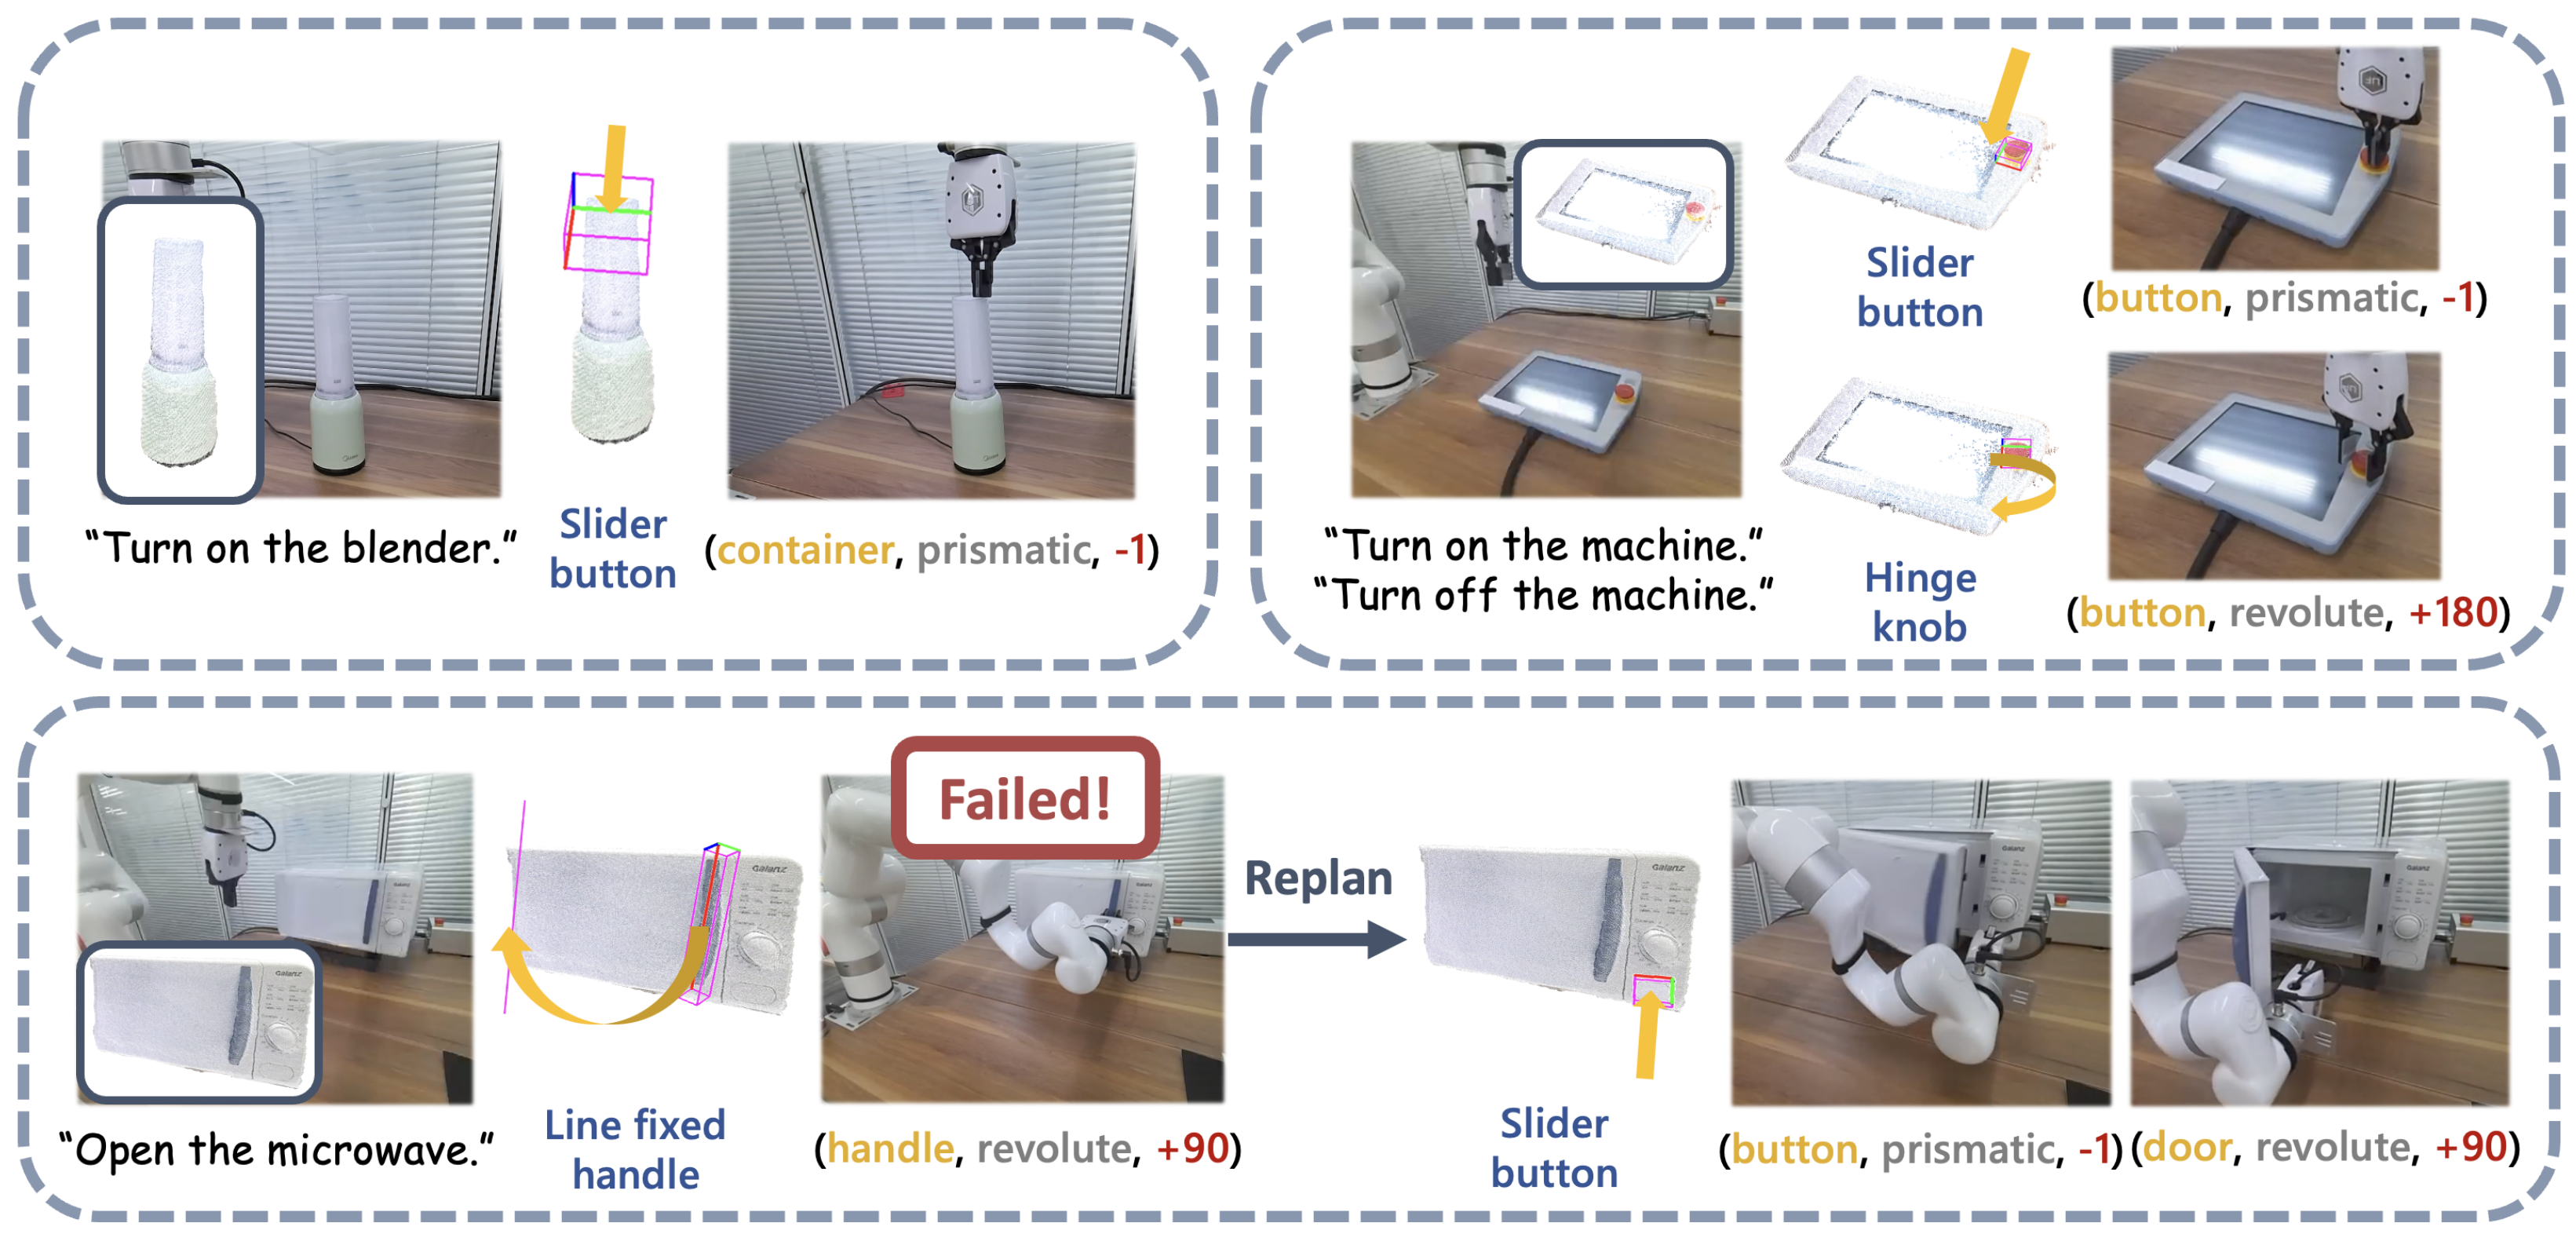
\includegraphics[width=1\linewidth]{figures/real_exp2.jpg}
    \caption{\textbf{Explanations of real-world results.}
    \textbf{Top:} "turn on the blender" and "turn on/off the machine". Our method accurately understands the part semantics and actions that are not aligned.
    \textbf{Bottom:} "Open the microwave". The mechanical structures of the microwave prevent the robot from directly pulling open the door but instead require the button to be pressed, resulting in a failure. However, our interactive feedback model can detect the failure and recognize that it should try pressing the button instead and subsequently complete the task.}
    \label{fig:exp_real_detail}
\end{figure}

\begin{figure*}
  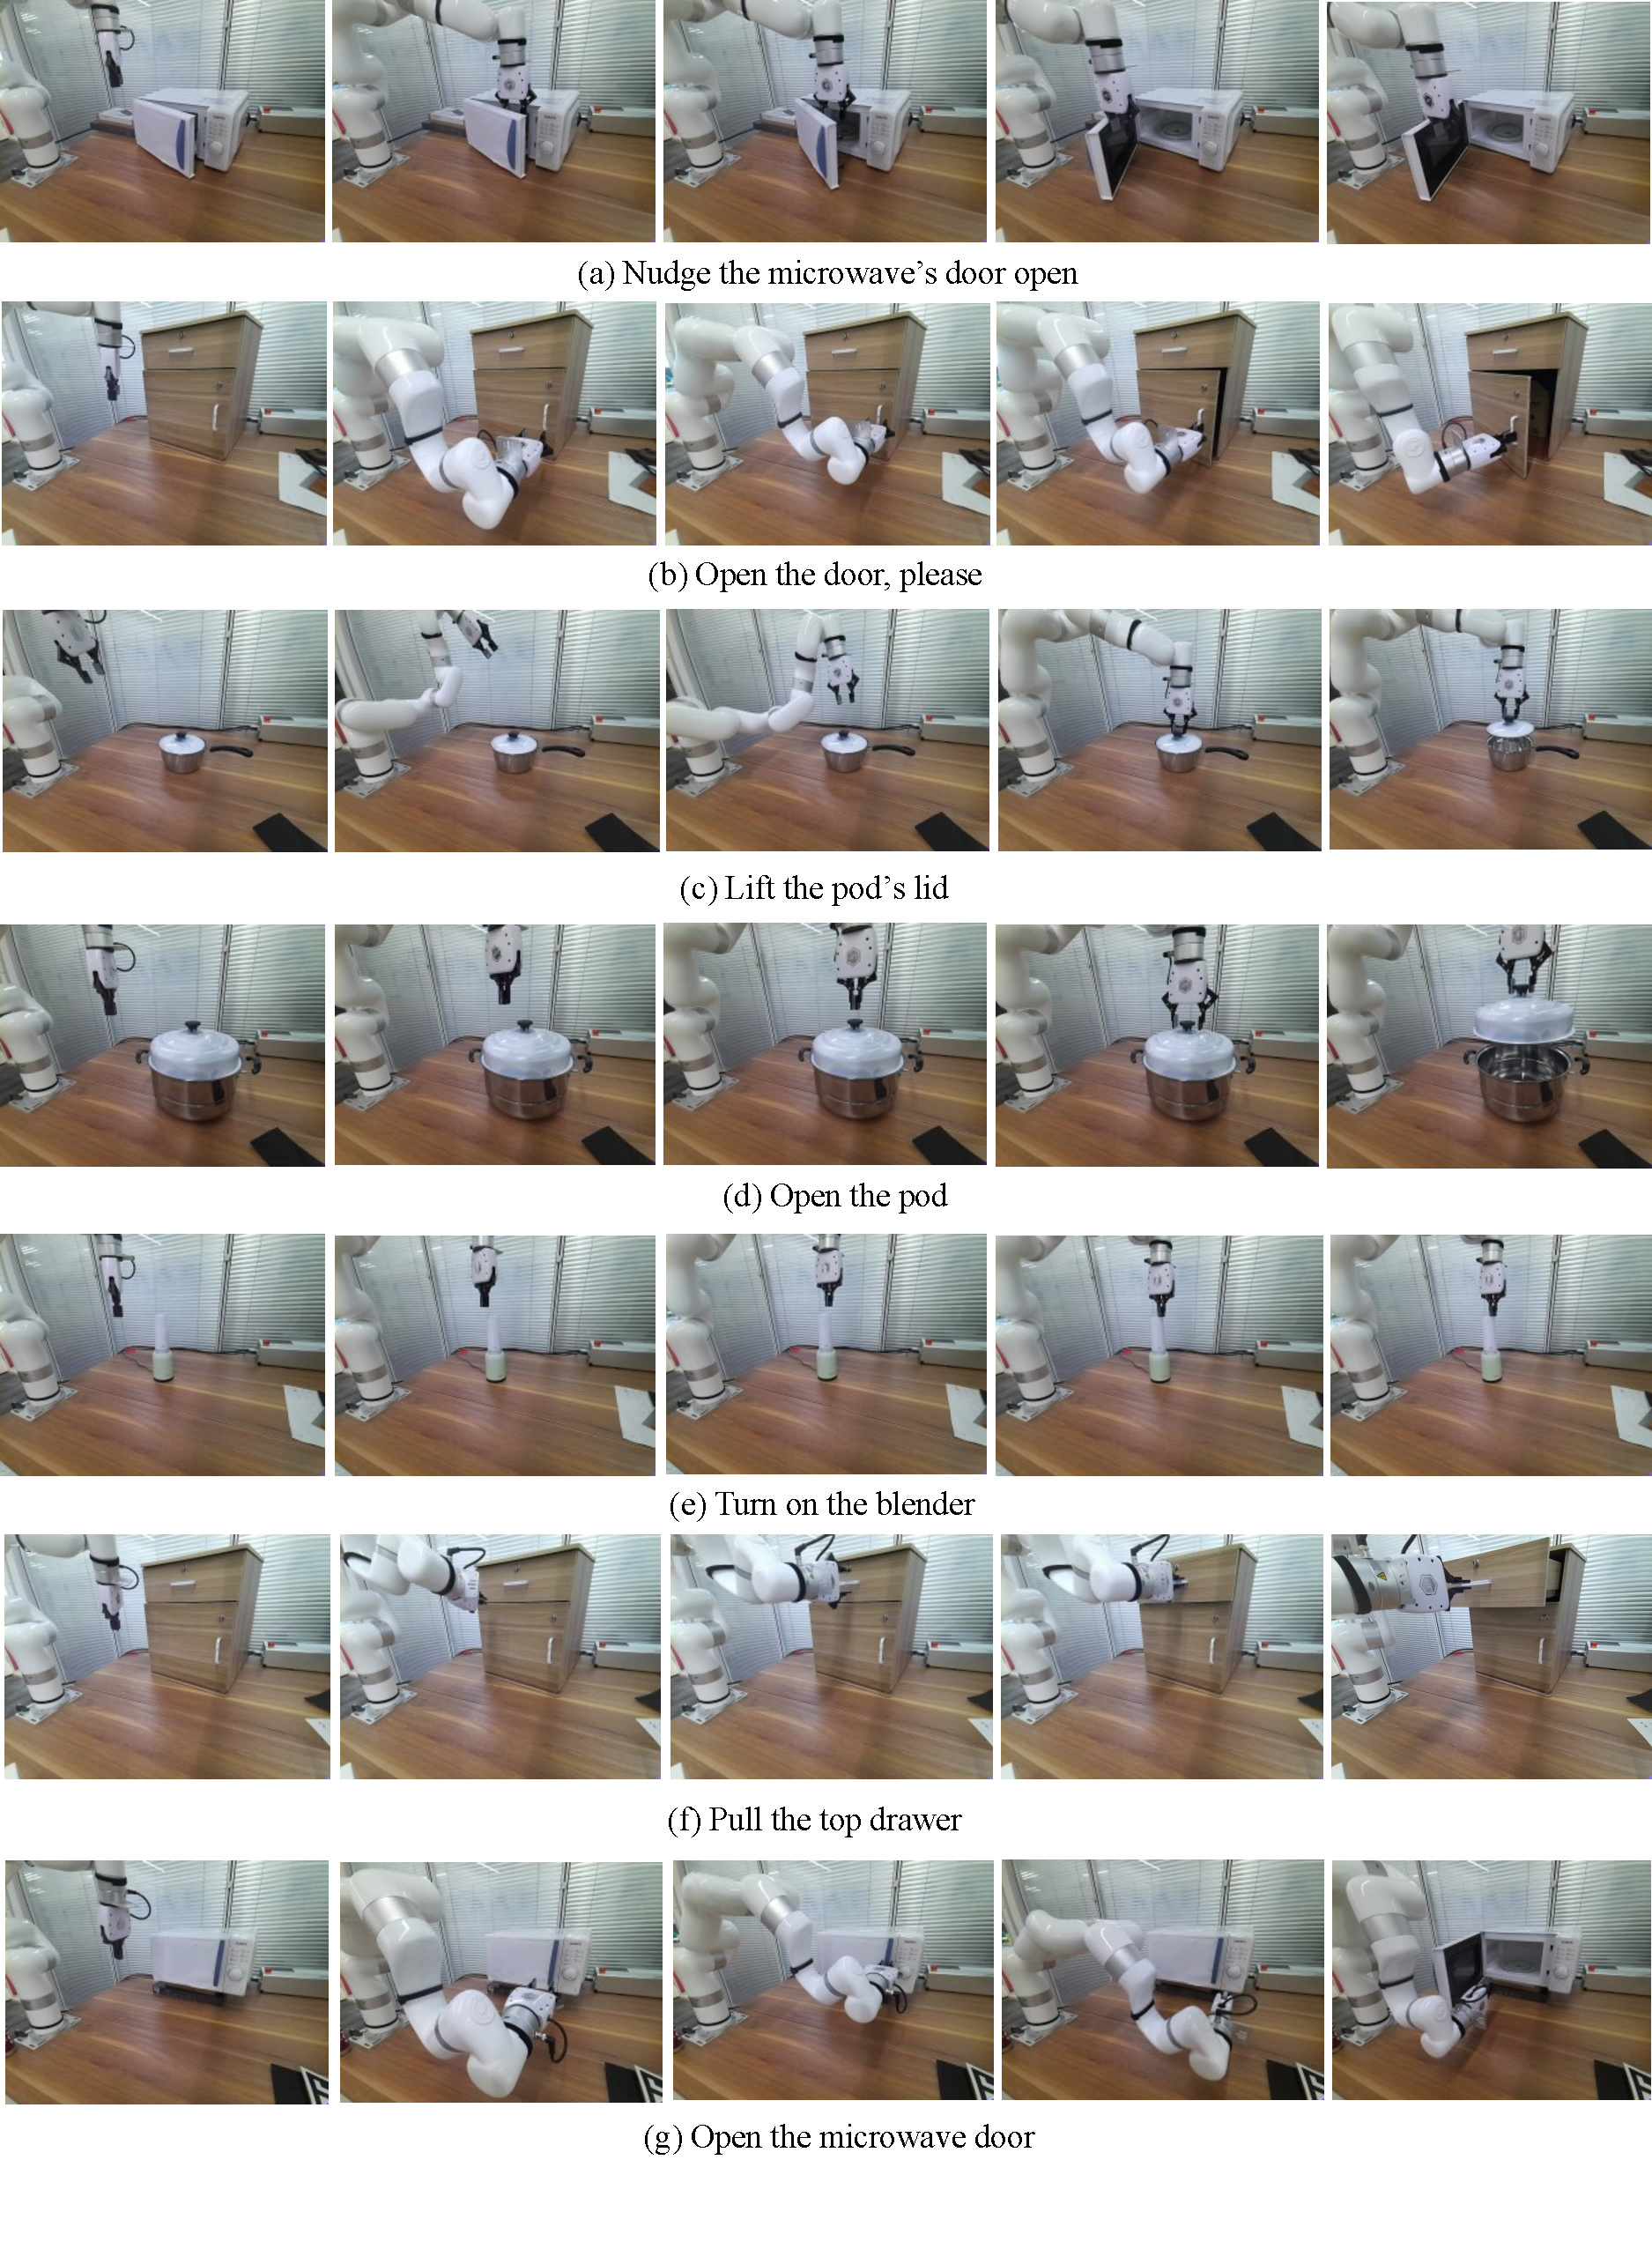
\includegraphics[width=\textwidth]{figures/real.pdf}
  \caption{\textbf{Real-robot results.} We show the keyframes of various tasks in our experiments. 
  More results can be found in the \SupplementaryMaterial.}
\end{figure*}


\subsection{Real-Robot Experiments}

\paragraph{Setup}
In our real-world experiments, we establish an experimental setup with the UFACTORY xArm 6 and several different articulated objects for manipulation.

\paragraph{Results}
Fig.~\ref{fig:exp_real_detail} shows our results on real-robot execution, and more results can be found in the \SupplementaryMaterial.
%
Three challenging cases are highlighted in Fig.~\ref{fig:exp_real_detail} with detailed explanations and intermediate outputs.
%
The top left is a blender whose top part is perceived as a container for containing juices but functions as a button to be pressed down. Our framework effectively links its semantic and action understandings and successfully executes the task.
%
The top right shows an emergency stop button for robots, which requires a press (down) to halt an operation and a rotation (up) to restart it. With the auxiliary input of the user manual, our method completes both of these two tasks.
%
The bottom shows a rather challenging case where the microwave door cannot be directly pulled open. Instead, it requires first pressing the button to initiate a slight door opening. In this case, our method first tries the most straightforward solution of pulling the door and fails. The interactive feedback module then detects this failure and informs the global planner to replan a second strategy that adapts to the current environment, finally completing the task.

%\TODO{One paragraph analyzing the numbers.}


\subsection{Generalizable Visual Perception}

\begin{table}[t]
\centering
\resizebox{0.49\textwidth}{!}{
\setlength{\tabcolsep}{1.5pt}
\begin{tabular}{l|c|cc|cc}
\toprule
    MOS $\uparrow$ & GAPartNet 
   & \begin{tabular}[c]{@{}c@{}}VLM\\ (Bard)  \end{tabular}  
   & \begin{tabular}[c]{@{}c@{}}\textbf{Ours}\\ (Bard)  \end{tabular}
   & \begin{tabular}[c]{@{}c@{}}VLM\\ (GPT4V)  \end{tabular}
   & \begin{tabular}[c]{@{}c@{}}\textbf{Ours}\\ (GPT4V)  \end{tabular} \\
\midrule
Part description & 3.8 & 4.1 & 6.3 & 7.2 & \textbf{9.6} \\        
% &8.8&4.4&\textbf{9.4}&&\\
Part accuracy & 8.7 & 4.0 & 6.5 & 6.9 & \textbf{9.5} \\       
% &6.6&7.9&\textbf{9.2}&&\\
Part state precision & 0.0 & 3.7 & 5.6 & 7.7 & \textbf{7.8} \\       
% &0.7&3.4&\textbf{6.8}&&\\
Object \& scene descr. & 0.0 & 2.7 & 6.2 & 6.4 & \textbf{8.0} \\   
% &0.5&\textbf{9.0}&\textbf{9.0}&&\\
Interaction info. & 0.3 & 7.3 & 7.6 & 7.6 & \textbf{8.7} \\      
% &0.4&1.2&\textbf{8.9}&&\\
Overall performance & 2.6 & 4.4 & 6.4 & 7.2 & \textbf{8.7} \\      
% &3.5&7.0&\textbf{9.4}&&\\
\bottomrule
\end{tabular}
}
\caption{\textbf{User study results for scene description.} We solicited volunteers to assess the quality of scene descriptions. Participants were tasked with evaluating the following aspects:
(1) Performance in the overall part description.
(2) Accuracy in the enumeration and naming of parts.
(3) Precision in part-state depiction.
(4) Depiction of objects and the overall scene.
(5) Description of interaction-related information.
(6) Overall performance.}
\label{tab:scene_result}
\end{table}



\begin{figure*}[t]
\begin{minipage}[c]{0.68\linewidth}
\resizebox{\columnwidth}{!}{%
  \begin{tabular}{l|cc|cc|cc|cc}
    \toprule
    Part Perception & \multicolumn{2}{c|}{\textbf{In-distribution}} & \multicolumn{2}{c|}{\textbf{Unseen states}} & \multicolumn{2}{c|}{\textbf{Unseen objects}} & \multicolumn{2}{c}{\textbf{Unseen categories}} \\
    Accuracy& AP@50     & mAP    & AP@50     & mAP    & AP@50              & mAP             & AP@50             & mAP             \\
    \midrule
    PointGroup\citep{jiang2020pointgroup} & 69.70 & 60.58 & 69.54 & 60.48 & 58.26 & 46.29 & 24.57 & 19.40 \\
    SoftGroup\citep{vu2022softgroup} & 69.59 & 60.54 & 70.02 & 59.59 & 59.20 & 47.10 & 28.18 & 22.50 \\
    AutoGPart\citep{liu2022autogpart} & 66.81 & 57.63 & 67.60 & 56.69 & 55.30 & 43.50 & 26.24 & 20.38 \\
    GAPartNet\citep{geng2022gapartnet} & 81.42 & \textbf{72.55} & 80.80 & 71.73 & 63.18 & 53.94 & 36.39 & 27.40 \\ %72.55	71.73	53.94	27.40
    PartGroundedSAM \citep{kirillov2023segany, oquab2023dinov2}   &73.73&61.75&72.36&62.02&66.25&38.64&41.59&28.45\\ %61.75	62.02	38.64	28.45
    \textbf{Ours}
    & \textbf{83.04} & \text{72.23} & \textbf{82.39} & \textbf{71.91} & \textbf{72.17} & \textbf{58.04} & \textbf{47.69} & \textbf{34.57} \\
    \bottomrule
\end{tabular}}
    \captionof{table}{\textbf{Part perception results.} We have curated a novel evaluation dataset for part perception, enriched with more comprehensive data. Our method is benchmarked against 3D point cloud-based techniques, including PointGroup\citep{jiang2020pointgroup}, SoftGroup\citep{vu2022softgroup}, AutoGPart\citep{liu2022autogpart}, and GAPartNet\citep{geng2022gapartnet}. In alignment with the 2D branch of our approach, we also employ SAM\citep{kirillov2023segany} and DINOv2\citep{oquab2023dinov2} to establish a 2D-centric baseline. For evaluation, we adopt AP@50 and mAP as our primary metrics.}
    \label{tab:perception_results}
\end{minipage}
\hfill %
\begin{minipage}[c]{0.3\linewidth}
    \centering
    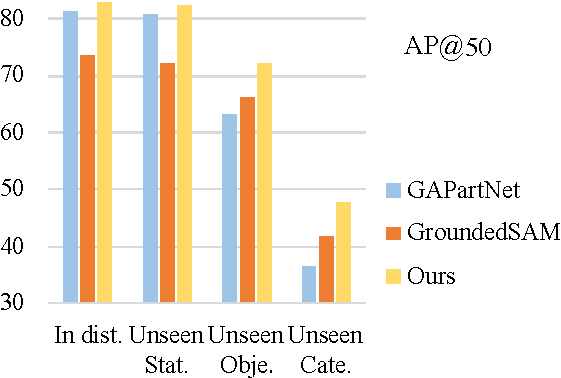
\includegraphics[width=0.98\linewidth, trim=0 .5cm 0 .5cm, clip]{figures/chart_percept.pdf}
    \caption{\textbf{Part perception results.}
    Our method consistently achieved the highest AP@50 score for each level of generalization.}
    \label{fig:3dcompare}
  \end{minipage}
  % \label{tab:baseline_wrapper}
\end{figure*}


As described in Sec. \ref{sec:method}, we design knowledge fusion mechanisms to join the force VLMs and small domain-specific models both in our context comprehension and part perception. In this section, we evaluate our intermediate results on scene description (Sec. \ref{sec:method:scene_percep}) and part perception (Sec. \ref{sec:grounding}) and show that our generalizable perception modules achieve a better balance between generalization and exactness compared to existing methods or its ablated versions.


\paragraph{Scene description (Sec. \ref{sec:method:scene_percep})}
In our instruction interpreter, a scene description is generated from the visual observations to inform the other modules of the scene context.
%
To evaluate the quality of scene descriptions generated by our method which joins the forces of generalist and specialist models, 
we curate an image dataset specifically for evaluating scene descriptions for manipulation purposes. The dataset includes 145 images from 15 object categories with varying part states.
%
We also designed six interaction-oriented metrics for assessing the qualities of the descriptions: part description, part accuracy, part state precision, object\&scene description, interaction-related information, and overall performance.
With these metrics, we can collect the Mean Opinion Score (MOS) through carefully designed user studies, as in \citep{gal2022image}.


We evaluate the scene descriptions generated by five methods:  (1) GAPart Model: detection results are translated into natural language descriptions through a human-crafted format; (2)(3) VLM (Bard, GPT-4V), craft descriptions from the input image using Bard and GPT-4V; (4)(5) Our methods (based on Bard and GPT-4V).
%
In the user study, participants are provided an image and the descriptions generated by the three methods at each time, and they are asked to rate the descriptions using a scale of 0-10 (with 10 being the best) according to the 6 metrics. 17 participants have been invited, and each person is asked to rate about 40 scenes on average.


Table~\ref{tab:scene_result} shows the results of this user study. We found that domain-specific models can hardly provide useful object and scene-level descriptions due to their lack of general knowledge. On the other hand, VLM provides rich context but lacks accuracy in domain-related information. Our method benefits from both of them and achieves much better performances by joining their strengths.

 

% We collect a dataset for scene description. We use three different methods to generate the scene description. The first is the GAPart Model. We use a human-designed format to translate detection results into a natural language description. The second method is directly using VLM, \ie Bard here, to generate a description for the input image. The third is our method.

% To evaluate the performance of the generated description, inspired by \citep{}, we introduce a user study and collect the Mean Opinion Score (MOS) on the evaluation under several metrics (see table \ref{xxx} for more details).




\paragraph{Part perception (Sec. \ref{sec:grounding})}
In our part perception task, we utilize a single RGBD image as input to predict part-related information, including part semantic segmentation, pose and state estimation. To evaluate the methods, we introduce a new benchmark for part perception tasks. In comparison with GAPartNet, our benchmark is more comprehensive and suitable for manipulation tasks. For instance, we incorporate a greater number of objects with closed parts, accounting for 12.5\%, which is not included in GAPartNet\citep{geng2022gapartnet}.
%
To enable the evaluation of generalizations at different levels, the test data are divided into 4 subsets: in-distribution, unseen (articulation) states, unseen objects, and unseen object categories.
% evaluate metrics
We use the average precision AP@50 and mAP as evaluation metrics for part segmentation, which are widely adopted in prior 3D semantic/instance segmentation benchmarks such as ScanNet\citep{dai2017scannet} and GAPartNet\citep{geng2022gapartnet},

Table \ref{tab:perception_results} presents the results of our method in comparison to various baselines for part perception. We consider GAPartNet\citep{geng2022gapartnet}, a modified version of PointGroup\citep{jiang2020pointgroup}, SoftGroup\citep{vu2022softgroup}, and AutoGPart \citep{liu2022autogpart} as our primary baselines. Additionally, we adapted GroundedSAM, rebranding it as PartGroundedSAM for this context. The performance metrics in Table \ref{tab:perception_results} indicate that our approach surpasses other baselines. Notably, we observed that methods based on 3D tend to under-perform on out-of-domain data, whereas 2D-centric methods yield subpar results for parts. Our methodology derives advantages from both the 2D and 3D realms, resulting in optimal performance and superior generalization capabilities.


% Table \ref{} presents our results, revealing several insights:
% \TODO{rewrite here}
% (1) Enhanced performance in 2D generalization.
% (2) Superior performance in the 3D domain.
% (3) A combined approach of 2D and 3D further bolsters performance.
% We build a benchmark to evaluate part perception. Compared with GAPartNet, we include more challenging perception tasks, \eg, we use more objects with closed part(12.5\%). To study the generalizability of our method, we evaluate part perception with four different level of generalizations (more details are in table \ref{xxx}).
% Following the previous 3D semantic instance segmentation benchmarks in ScanNet\citep{} and GAPartNet\citep{}, we use the widely adopted metric average precision to evaluate the performance of part segmentation.

% The results in table \ref{} shows that (1) 2d generalization (2) 3d domain performance higher (3) combine 2d and 3d improve performance.

% \begin{table*}[ht]
% \centering
% % \setlength\tabcolsep{2pt}
% % \vspace{-1.5em}
% \renewcommand\arraystretch{0.9}
% \resizebox{.99\textwidth}{!}{
% \begin{tabular}
% {c|c|ccccccccccc}
% \hline

% && Ln.F.Hl. & Rd.F.Hl. & Hg.Hl. & Hg.Ld.& Sd.Ld.  & Sd.Bn  & Sd.Dw. & Hg.Dr. & Hg.Kb. &Avg.AP
% % \begin{tabular}[c]{@{}c@{}} \\\end{tabular} 
% & Avg.AP50
% && Ln.F.Hl. & Rd.F.Hl. & Hg.Hl. & Hg.Ld.& Sd.Ld.  & Sd.Bn  & Sd.Dw. & Hg.Dr. & Hg.Kb. &Avg.AP
% % \begin{tabular}[c]{@{}c@{}} \\\end{tabular} 
% & Avg.AP50
% % \begin{tabular}[c]{@{}l@{}}\\ \end{tabular} 
% \\ \hline
% \multirow{4}{*}{Seen (\%)}   & PG\citep{jiang2020pointgroup} &86.1 &23.0 &84.6 &80.01&88.3 &49.3 &62.6 &92.8 &34.6 &57.3 &66.8 \\ %\cline{2-13} 
%                         & SG\citep{vu2022softgroup} & 57.8 & \textbf{93.6} & 81.2 & 76.0 & 89.3 & 25.2 & 50.8 & 93.9 & 51.5 & 58.5 & 68.8 \\ %\cline{2-13} 
%                         & AGP\citep{liu2022autogpart} &86.8 &20.3  &87.7 &79.7  &89.4  &62.3   &61.6  &92.5  & 16.7 & 57.2 &66.3 \\ %\cline{2-13} 
%                         % & AutoGPart  & & & & & & & & & & & \\ \cline{2-13} 
%                         & GAPartNet\citep{geng2022gapartnet}       &\textbf{89.2} &54.9 &\textbf{90.4} &\textbf{84.8} &\textbf{89.8} &\textbf{66.7} &\textbf{67.2} &\textbf{94.7} &\textbf{52.9} &\textbf{67.6} &\textbf{76.5} \\ 
%                         & PartGroundedSAM       &\textbf{89.2} &54.9 &\textbf{90.4} &\textbf{84.8} &\textbf{89.8} &\textbf{66.7} &\textbf{67.2} &\textbf{94.7} &\textbf{52.9} &\textbf{67.6} &\textbf{76.5} \\ 
%                         & Ours       &\textbf{89.2} &54.9 &\textbf{90.4} &\textbf{84.8} &\textbf{89.8} &\textbf{66.7} &\textbf{67.2} &\textbf{94.7} &\textbf{52.9} &\textbf{67.6} &\textbf{76.5} \\ \hline
% % \multirow{4}{*}{Unseen (\%)} & PG\citep{jiang2020pointgroup} &32.44 &\textbf{}9.8 &2.1 &26.8 &0.0 &42.6 &57.0 &63.9 &1.7 &21.9 &26.3 \\ %\cline{2-13} 
% %                         & SG\citep{vu2022softgroup} & 25.8 & 5.0 & 0.4 & 33.9 & 0.6 & \textbf{51.5} & 51.2 & \textbf{}69.0 & 12.1 & 22.0 & 27.7 \\ %\cline{2-13} 
% %                         % & AutoGPart  & \multicolumn{1}{l|}{} & \multicolumn{1}{l|}{} & \multicolumn{1}{l|}{} & \multicolumn{1}{l|}{} & \multicolumn{1}{l|}{} & \multicolumn{1}{l|}{} & \multicolumn{1}{l|}{} &        &        &    &    \\ \cline{2-13} 
% %                         & AGP\citep{liu2022autogpart} &\textbf{45.6} &4.8  &\textbf{3.1}  &34.3 &0.0  &47.8 &64.1 &63.1  &11.5  &25.7  &30.5  \\ %\cline{2-13} 
% %                         & GAPartNet& {\textbf{45.6}} & {\textbf{40.0}} & {\textbf{3.1}} & {\textbf{40.2}} & {\textbf{5.0}} & \multicolumn{1}{c}{\textbf{}49.1} & \multicolumn{1}{c}{\textbf{64.2}} &\textbf{69.1} &\textbf{23.4}&\textbf{32.0}  &\textbf{37.2}  \\ 
% %                         & PartGroundedSAM       &\textbf{89.2} &54.9 &\textbf{90.4} &\textbf{84.8} &\textbf{89.8} &\textbf{66.7} &\textbf{67.2} &\textbf{94.7} &\textbf{52.9} &\textbf{67.6} &\textbf{76.5} \\ 
% %                         & Ours       &\textbf{89.2} &54.9 &\textbf{90.4} &\textbf{84.8} &\textbf{89.8} &\textbf{66.7} &\textbf{67.2} &\textbf{94.7} &\textbf{52.9} &\textbf{67.6} &\textbf{76.5} \\ \hline
% \end{tabular}
% }
% % \vspace{-2mm}
% \caption{\textbf{Results of Part Segmentation on Seen Object Categories and Unseen Object Categories in terms of Per-part-class AP50 (\%), Average AP50 (\%), and Average AP (\%).} Ln.=Line. F.=Fixed. Rd.=Round. Hl.=Handle. Ld.=Lid. Bn.=Button. Dw.=Drawer. Dr.=Door. Kb.=Knob.  PG=PointGroup\citep{jiang2020pointgroup}. SG=SoftGroup\citep{vu2022softgroup}.
% AGP=baseline modified from AutoGPart\citep{liu2022autogpart}.}
% \label{table:mainres}
% \vspace{-3mm}
% \end{table*}

% \TODO{Quantitative Results: Compare with Baseline; Ablation}







